\paragraph{}En este proceso, el usuario administrador de centro puede crear,
consultar, modificar o borrar asignaturas de la aplicación.

\paragraph{}La figura \ref{diagramaNivel4-AdministrarAsignaturas-admCentro}
muestra el nivel de abstracción 4: Administrar asignaturas (módulo Administrador
de centro).

  \begin{figure}[!ht]
    \begin{center}
      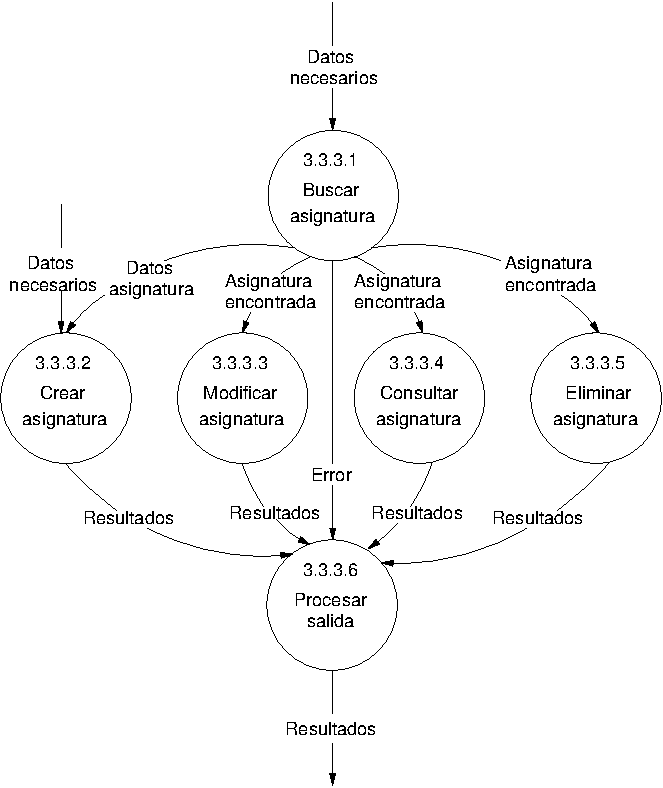
\includegraphics[]{08.Analisis_Funcional/8.2.DFDs/Niveles/Nivel4/AdministradorCentro/AdministrarAsignaturas/Diagramas/nivel4-AdministrarAsignaturas.pdf}
      \caption{Nivel de abstracción 4: Administrar asignaturas (módulo Administrador de centro).}
      \label{diagramaNivel4-AdministrarAsignaturas-admCentro}
    \end{center}
  \end{figure}
